% ============================================================================
% RESULTADOS — planejamento de rotas
% Chamado em partes/textuais/resultados.tex.
% Dados brutos: DroneSTM32/docs/resultados_rotas/pc/ (resultados.csv,
% resumo.json, limite_exato.json, convergencia.json).
% Figuras: DroneSTM32/tools/pi/rotas_figuras_tcc.py.
% ============================================================================

\section{PLANEJAMENTO DE ROTAS}\label{sec:res_rotas}

Esta seção apresenta os resultados do \textit{benchmark} descrito na Seção~\ref{subsubsec:rotas_benchmark}: o limite de viabilidade dos métodos exatos, a qualidade e o tempo de cálculo das rotas, a convergência do algoritmo genético, uma investigação complementar da busca local 2-opt, a execução das rotas no controlador de voo e a execução do AG no Raspberry Pi Zero W. O \textit{benchmark} completo levou 21~min e produziu a assinatura SHA-256 \texttt{af4482d38e122be7\ldots{}dcb978532f0}.

% ----------------------------------------------------------------
\subsection{Limite de viabilidade dos métodos exatos}\label{subsec:res_rotas_limite}
% ----------------------------------------------------------------

A Tabela~\ref{tab:rotas_limite_fb} apresenta os tempos da força bruta. A memória do processo permaneceu constante em cerca de 22~MB, ocupados pelo próprio interpretador Python; o limite do método é exclusivamente o tempo, que cresce por um fator próximo de $N$ a cada ponto adicionado. Com 10 pontos, a instância é resolvida em 1,5~s; com 11, em 18~s; a partir de 12, a extrapolação indica minutos, dias e, com 20 pontos, dezenas de milhares de anos.

\begin{table}[H]
    \centering
    \caption{Tempo da força bruta por instância.}
    \label{tab:rotas_limite_fb}
    \small
    \renewcommand{\arraystretch}{1.2}
    \begin{tabular}{cccc}
        \hline
        \textbf{Pontos ($N$)} & \textbf{Ordens avaliadas} & \textbf{Tempo} & \textbf{Origem} \\
        \hline
        5 & 120 & 0,1~ms & medido \\
        8 & 40\,320 & 14~ms & medido \\
        9 & 362\,880 & 0,15~s & medido \\
        10 & 3\,628\,800 & 1,5~s & medido \\
        11 & 39\,916\,800 & 18~s & medido \\
        12 & $4{,}8 \times 10^{8}$ & $\approx$ 3~min & previsto \\
        13 & $6{,}2 \times 10^{9}$ & $\approx$ 43~min & previsto \\
        15 & $1{,}3 \times 10^{12}$ & $\approx$ 6~dias & previsto \\
        17 & $3{,}6 \times 10^{14}$ & $\approx$ 4,7~anos & previsto \\
        20 & $2{,}4 \times 10^{18}$ & $\approx$ 32~mil anos & previsto \\
        \hline
    \end{tabular}
    \par\vspace{0.2cm}
    \footnotesize Fonte: elaborado pelos autores (2026).
\end{table}

O Held-Karp (Tabela~\ref{tab:rotas_limite_hk}) resolve as mesmas instâncias muito mais rápido, mas o tempo aproximadamente dobra a cada ponto (fator medido entre 2,0 e 2,4) e a memória acompanha o número de estados $N \cdot 2^N$. Com 22 pontos, a instância levou de 59 a 64~s em duas medições, com 806~MB; com 23, de 125 a 131~s e 1,7~GB. Com 24 pontos, a memória necessária (3,6~GB) ocupa praticamente toda a RAM livre do computador, e com 25 (7,5~GB) supera a RAM total de 7,3~GB, o que torna o método impossível nessa máquina, independentemente do tempo disponível.

\begin{table}[H]
    \centering
    \caption{Tempo e memória do Held-Karp por instância.}
    \label{tab:rotas_limite_hk}
    \small
    \renewcommand{\arraystretch}{1.2}
    \begin{tabular}{ccccc}
        \hline
        \textbf{Pontos ($N$)} & \textbf{Tempo} & \textbf{Memória} & \textbf{Origem} & \textbf{Situação} \\
        \hline
        15 & 0,24~s & 22~MB & medido & viável \\
        18 & 2,6~s & 54~MB & medido & viável \\
        20 & 12,5~s & 194~MB & medido & viável \\
        21 & 26~s & 391~MB & medido & viável \\
        22 & 59 a 64~s & 806~MB & medido & último no comparativo \\
        23 & 125 a 131~s & 1,7~GB & medido & fora do comparativo \\
        24 & $\approx$ 5~min & 3,6~GB & previsto & ocupa a RAM livre \\
        25 & $\approx$ 10~min & 7,5~GB & previsto & excede a RAM total \\
        30 & $\approx$ 8~h & 290~GB & previsto & impossível \\
        \hline
    \end{tabular}
    \par\vspace{0.2cm}
    \footnotesize Fonte: elaborado pelos autores (2026).
\end{table}

A Figura~\ref{fig:rotas_tempo_resolver} reúne os tempos em escala logarítmica. Os marcadores indicam valores medidos, e as linhas tracejadas, valores previstos pelos modelos de crescimento. Os dois métodos exatos aparecem como curvas de crescimento exponencial, muito mais íngreme na força bruta; o guloso e o algoritmo genético crescem de forma polinomial e permanecem, em toda a faixa, abaixo de 1~ms e de 0,5~s, respectivamente. A Figura~\ref{fig:rotas_memoria} compara a memória do Held-Karp com a do AG: no Raspberry Pi Zero W, com 512~MB para todo o sistema, a tabela do Held-Karp ultrapassa metade da RAM a partir de 21 pontos, enquanto o AG não chega a 0,1~MB com 30 pontos.

\begin{figure}[H]
    \centering
    \caption{Tempo para resolver uma instância, por número de pontos, no computador Intel Core i5-9300HF.}
    \label{fig:rotas_tempo_resolver}
    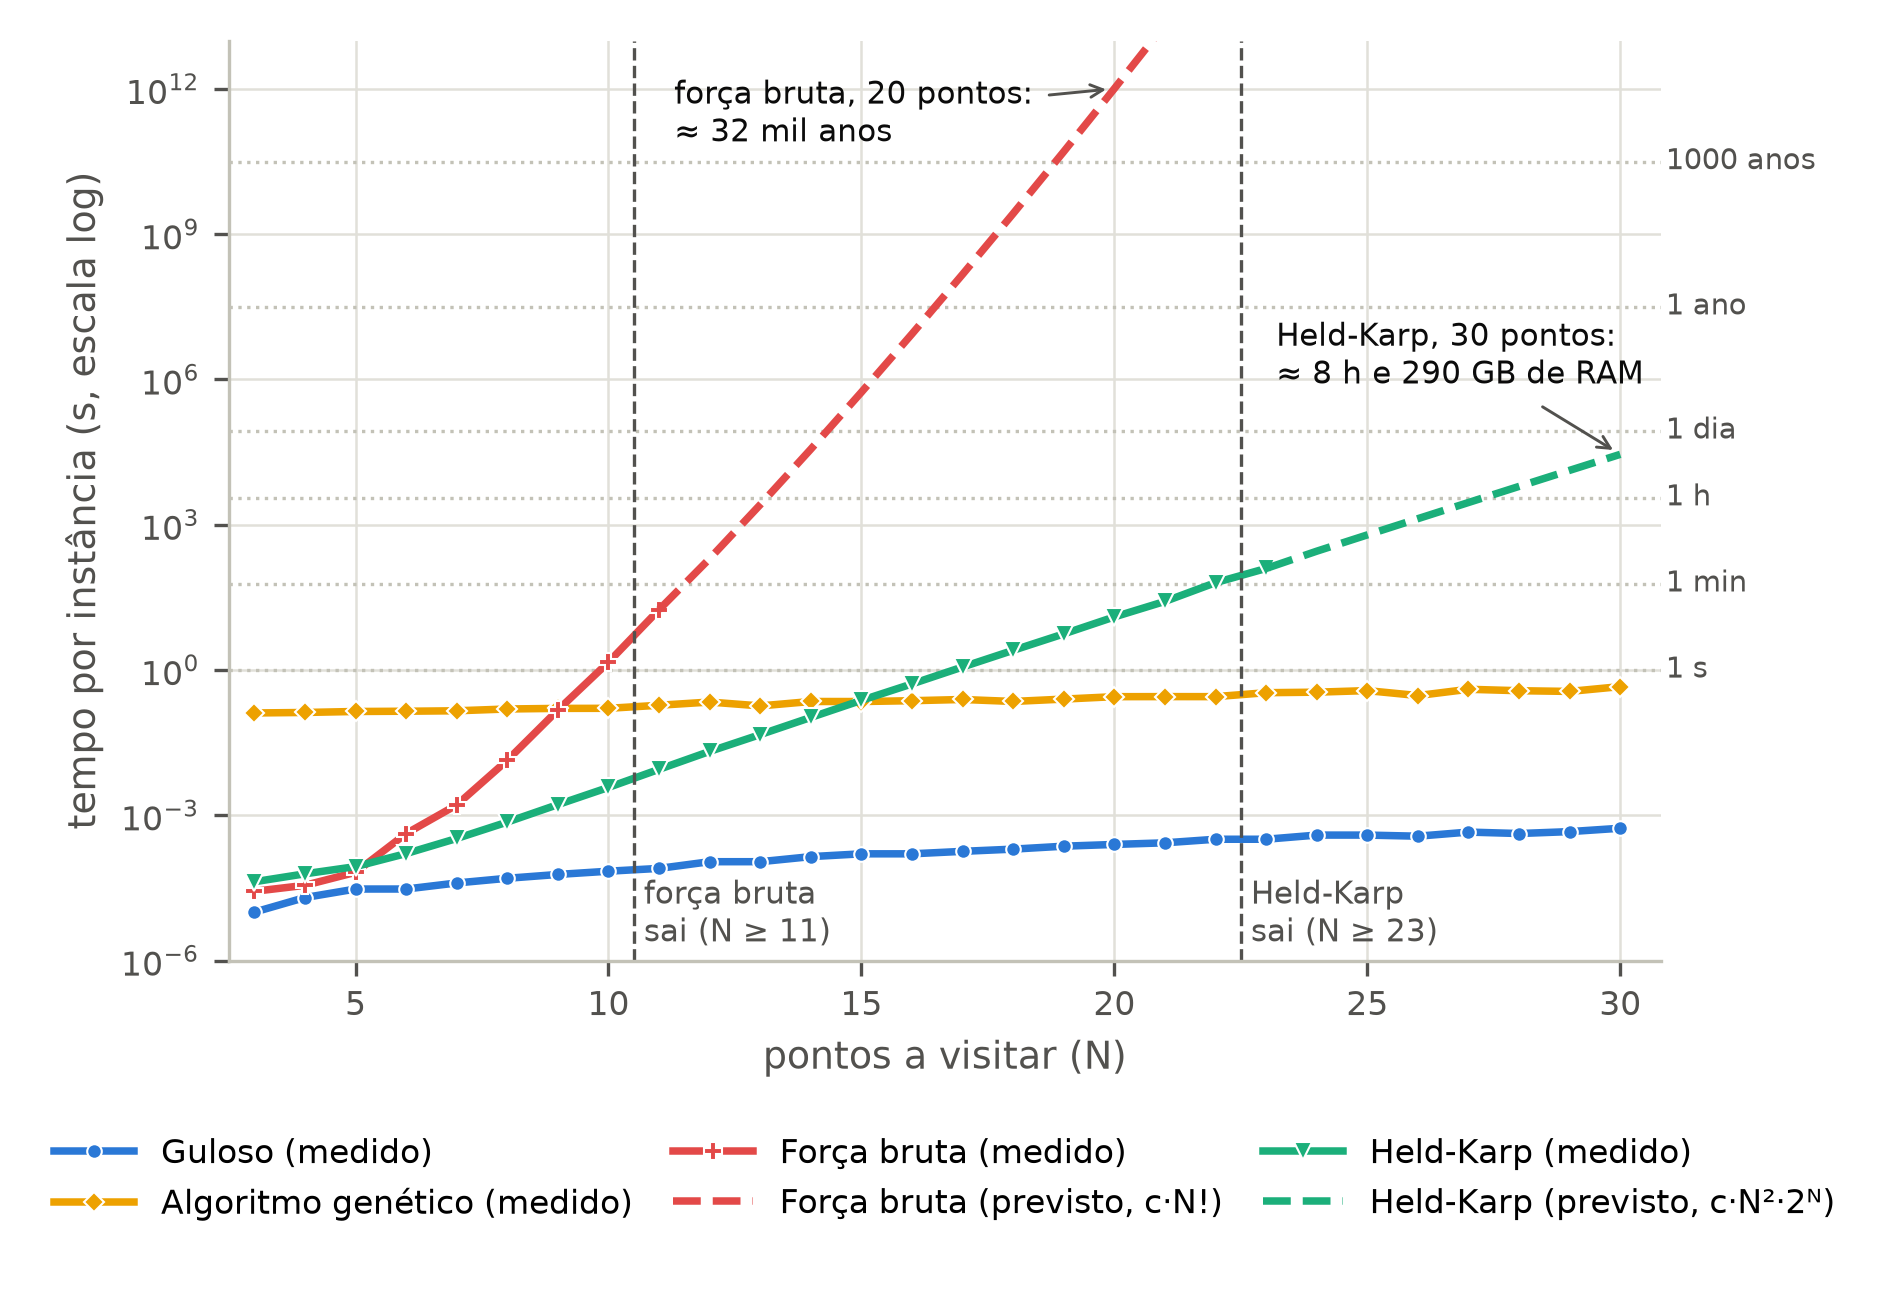
\includegraphics[width=\textwidth]{images/rotas/tempo_resolver.png}
    \fonte{elaborado pelos autores (2026).}
\end{figure}

\begin{figure}[H]
    \centering
    \caption{Memória necessária pelo Held-Karp e pelo algoritmo genético, por número de pontos.}
    \label{fig:rotas_memoria}
    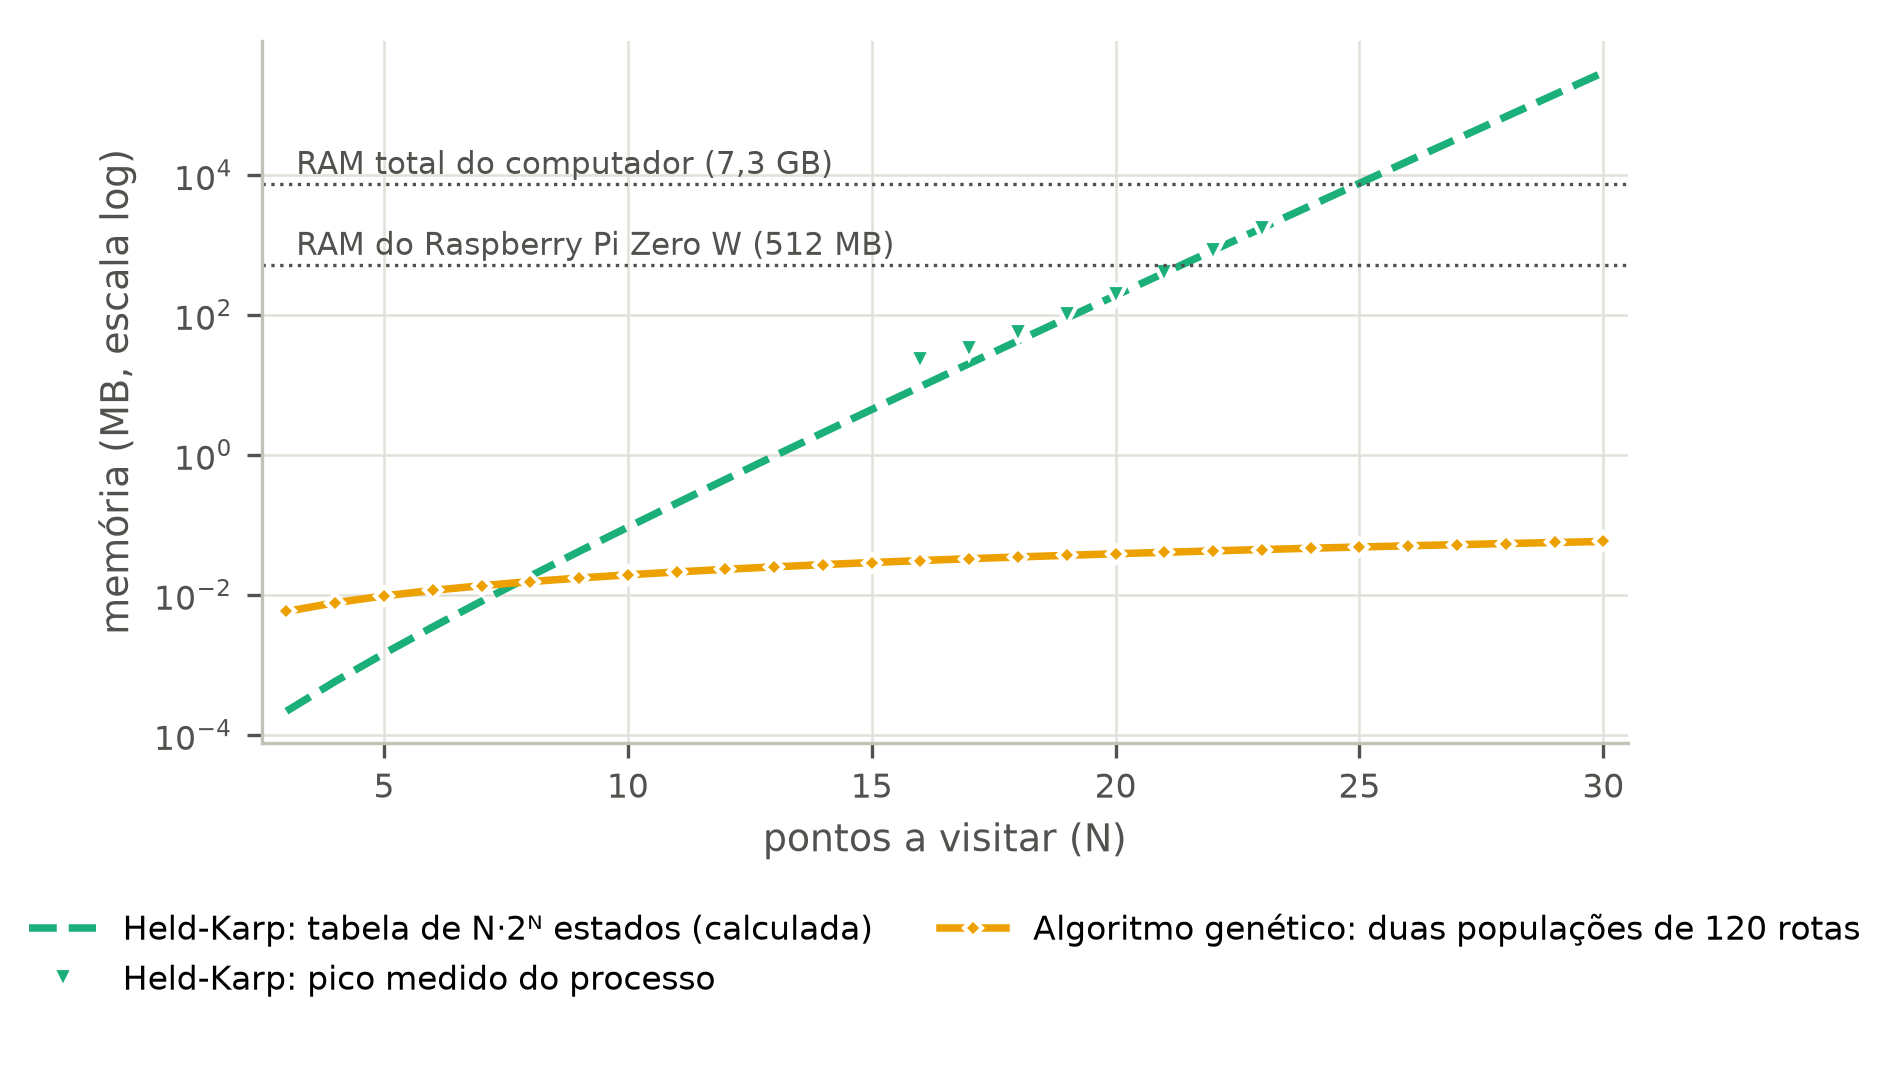
\includegraphics[width=\textwidth]{images/rotas/memoria_exato.png}
    \fonte{elaborado pelos autores (2026).}
\end{figure}

Com o critério da Seção~\ref{subsubsec:rotas_viabilidade}, cada método exato deixa o comparativo em um ponto diferente, o que divide os resultados em três faixas (Tabela~\ref{tab:rotas_fases}). Nas 80 instâncias em que os dois métodos exatos rodaram, os custos coincidiram em todas, o que confirma a implementação do Held-Karp.

\begin{table}[H]
    \centering
    \caption{Algoritmos executados em cada faixa de número de pontos.}
    \label{tab:rotas_fases}
    \small
    \renewcommand{\arraystretch}{1.25}
    \begin{tabular}{cccccc}
        \hline
        \textbf{Pontos ($N$)} & \textbf{Aleatório} & \textbf{Guloso} & \textbf{AG} & \textbf{Força bruta} & \textbf{Held-Karp} \\
        \hline
        3 a 10 & sim & sim & sim & sim & sim \\
        11 a 22 & sim & sim & sim & não & sim \\
        23 a 30 & sim & sim & sim & não & não \\
        \hline
    \end{tabular}
    \par\vspace{0.15cm}
    \footnotesize A força bruta sai com 11 pontos (18~s por instância e $\approx$ 3~min com 12); o Held-Karp sai com 23 (mais de 2~min e 1,7~GB) e não cabe na memória a partir de 25.\\
    Fonte: elaborado pelos autores (2026).
\end{table}

% ----------------------------------------------------------------
\subsection{Qualidade das rotas}\label{subsec:res_rotas_qualidade}
% ----------------------------------------------------------------

A Figura~\ref{fig:rotas_qualidade} apresenta a qualidade média das rotas, isto é, a razão entre o comprimento da rota de referência e o da rota obtida: 100\% corresponde à rota ótima (ou à melhor conhecida, acima de 22 pontos), e quanto maior o valor, melhor a rota. O AG manteve qualidade entre 96,5\% e 100\% em toda a faixa, o guloso entre 85\% e 94\%, e a ordem aleatória caiu de 74\% para 33\% com o aumento de $N$. As distâncias médias correspondentes estão na Tabela~\ref{tab:rotas_distancia}.

\begin{figure}[H]
    \centering
    \caption{Qualidade média das rotas, em relação à rota ótima ou à melhor conhecida (10 instâncias por $N$).}
    \label{fig:rotas_qualidade}
    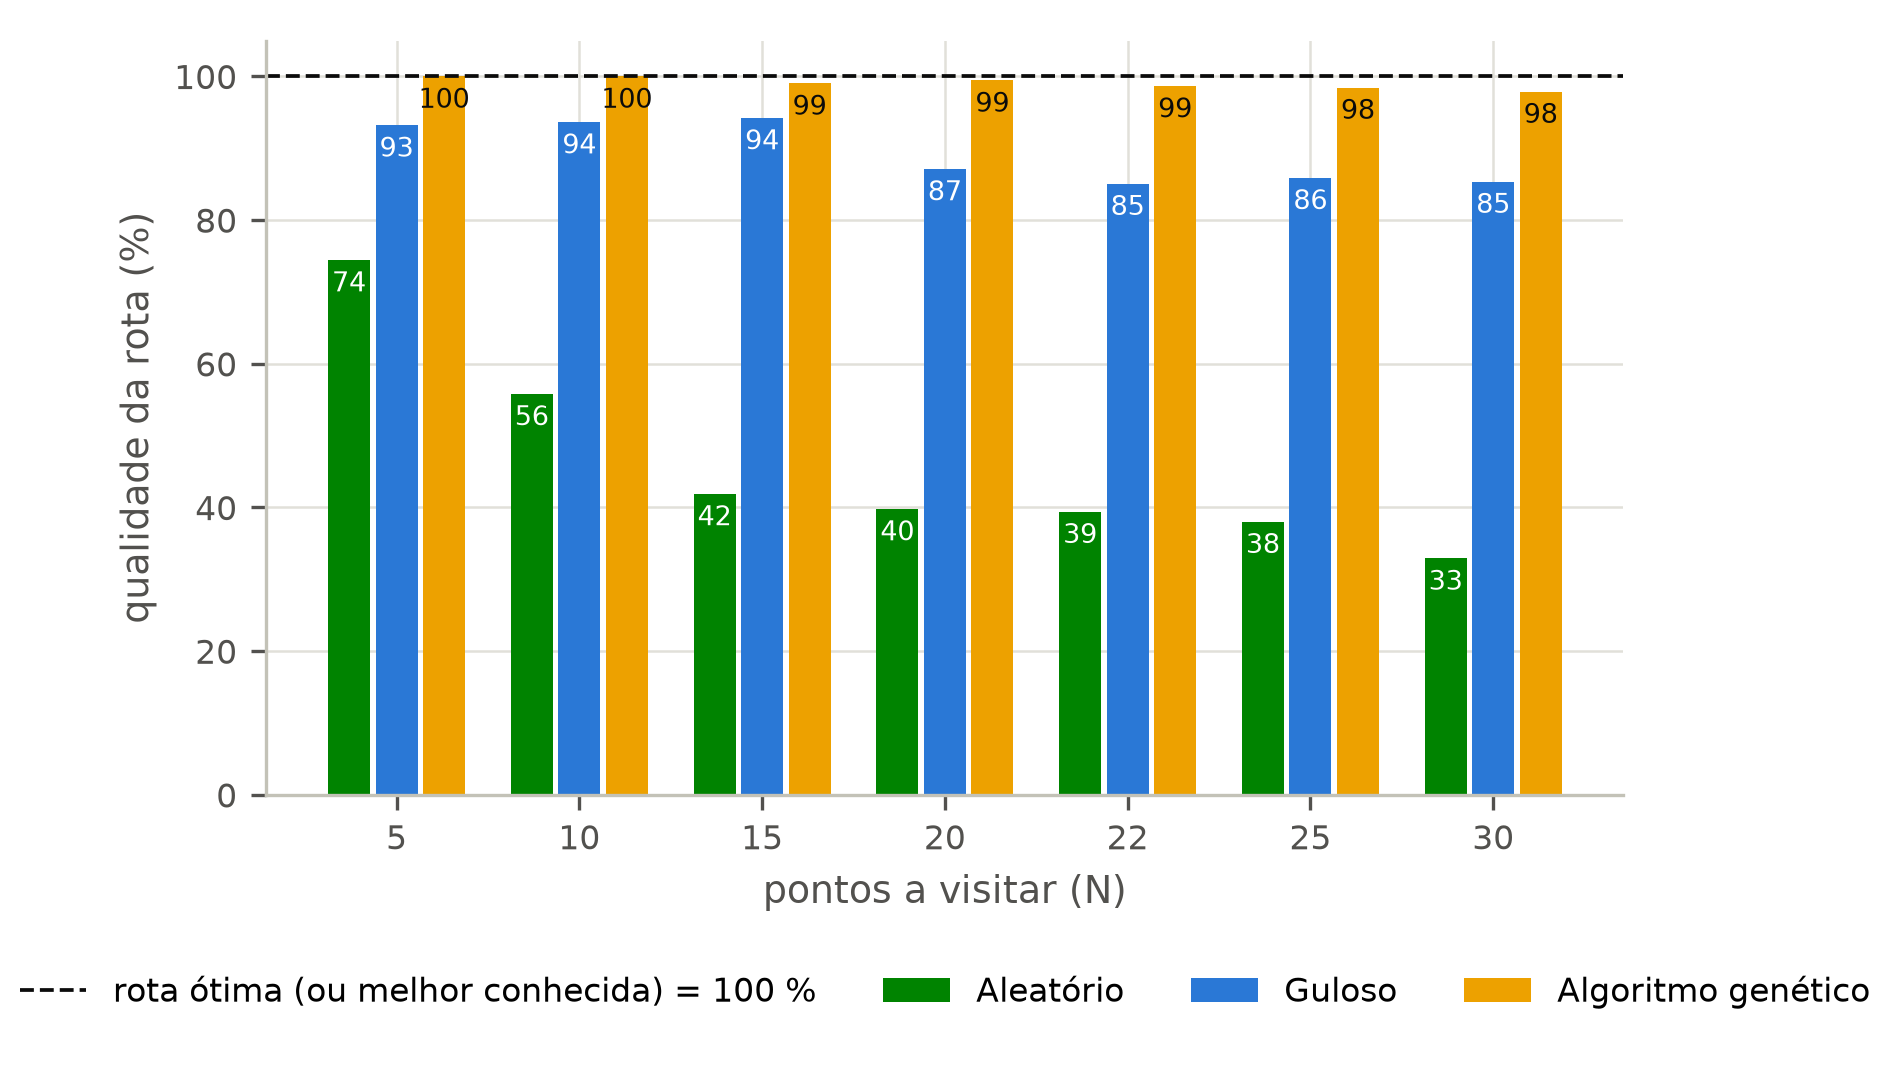
\includegraphics[width=\textwidth]{images/rotas/qualidade_rotas.png}
    \fonte{elaborado pelos autores (2026).}
\end{figure}

\begin{table}[H]
    \centering
    \caption{Distância média do circuito, em metros (10 instâncias por $N$).}
    \label{tab:rotas_distancia}
    \small
    \renewcommand{\arraystretch}{1.2}
    \begin{tabular}{cccccc}
        \hline
        \textbf{$N$} & \textbf{Aleatório} & \textbf{Guloso} & \textbf{AG} & \textbf{Força bruta} & \textbf{Held-Karp} \\
        \hline
        5 & 18,86 & 14,86 & 13,78 & 13,78 & 13,78 \\
        10 & 35,59 & 21,04 & 19,64 & 19,64 & 19,64 \\
        15 & 54,52 & 24,26 & 22,98 & --- & 22,76 \\
        20 & 65,12 & 29,82 & 25,94 & --- & 25,79 \\
        22 & 68,38 & 31,91 & 27,30 & --- & 26,93 \\
        25 & 77,76 & 34,34 & 29,76 & --- & --- \\
        30 & 98,44 & 38,04 & 32,96 & --- & --- \\
        \hline
    \end{tabular}
    \par\vspace{0.2cm}
    \footnotesize Fonte: elaborado pelos autores (2026).
\end{table}

A Tabela~\ref{tab:rotas_gap} agrupa o \textit{gap} e os acertos por faixa. Até 10 pontos, o AG obteve o ótimo global em todas as 80 instâncias; entre 11 e 22, em 70 de 120, com \textit{gap} médio de 0,85\%; entre 23 e 30, ficou em média 2,2\% acima da melhor rota conhecida. O guloso perdeu de 6,6\% a 18,3\% em média, chegando a 37\% em instâncias desfavoráveis.

\begin{table}[H]
    \centering
    \caption{\textit{Gap} médio, \textit{gap} máximo e acertos da referência, por faixa de $N$.}
    \label{tab:rotas_gap}
    \small
    \renewcommand{\arraystretch}{1.25}
    \setlength{\tabcolsep}{4pt}
    \begin{tabular}{lccc}
        \hline
        \textbf{Algoritmo} & \textbf{3 a 10 (ótimo)} & \textbf{11 a 22 (ótimo)} & \textbf{23 a 30 (melhor conhecida)} \\
        \hline
        Aleatório & 49,3\% (127,4\%) $\cdot$ 6/80 & 132,0\% (198,7\%) $\cdot$ 0/120 & 182,4\% (264,7\%) $\cdot$ 0/80 \\
        Guloso & 6,6\% (28,6\%) $\cdot$ 11/80 & 9,7\% (31,7\%) $\cdot$ 1/120 & 18,3\% (36,9\%) $\cdot$ 0/80 \\
        Algoritmo genético & 0,00\% (0,00\%) $\cdot$ 80/80 & 0,85\% (9,6\%) $\cdot$ 70/120 & 2,2\% (7,7\%) $\cdot$ 20/80 \\
        \hline
    \end{tabular}
    \par\vspace{0.15cm}
    \footnotesize Formato: \textit{gap} médio (\textit{gap} máximo) $\cdot$ instâncias em que a referência foi obtida.\\
    Fonte: elaborado pelos autores (2026).
\end{table}

A comparação instância a instância está na Tabela~\ref{tab:rotas_confronto}, em que cada célula indica em quantas das 280 instâncias o algoritmo da linha obteve rota mais curta que o da coluna. O AG superou o guloso em 262 instâncias e foi superado em 6; a ordem aleatória nunca superou o AG.

\begin{table}[H]
    \centering
    \caption{Instâncias, entre 280, em que o algoritmo da linha obteve rota mais curta que o da coluna.}
    \label{tab:rotas_confronto}
    \small
    \renewcommand{\arraystretch}{1.25}
    \begin{tabular}{lccc}
        \hline
        & \textbf{Aleatório} & \textbf{Guloso} & \textbf{AG} \\
        \hline
        \textbf{Aleatório} & --- & 9 & 0 \\
        \textbf{Guloso} & 270 & --- & 6 \\
        \textbf{AG} & 274 & 262 & --- \\
        \hline
    \end{tabular}
    \par\vspace{0.15cm}
    \footnotesize Empates (rotas de mesmo comprimento): aleatório e guloso, 1; aleatório e AG, 6; guloso e AG, 12.\\
    Fonte: elaborado pelos autores (2026).
\end{table}

As Figuras~\ref{fig:rotas_3d_n10} a \ref{fig:rotas_3d_n25} mostram as rotas em 3D de três instâncias. Com 10 e 20 pontos, o Held-Karp fornece o ótimo global, e o AG obtém exatamente a mesma rota, enquanto o guloso fica 26,1\% e 30,7\% acima, respectivamente. Com 25 pontos, o Held-Karp não pode ser executado, e o ótimo global é desconhecido. É nesse cenário que o \textit{benchmark} se mostra necessário: como o AG obteve o ótimo ou ficou próximo dele em todas as faixas em que o ótimo era conhecido, sua rota de 30,35~m é adotada como solução de referência prática, contra 34,14~m do guloso e 89,61~m da ordem aleatória.

\begin{figure}[H]
    \centering
    \caption{Rotas de 10 pontos obtidas pelos quatro algoritmos.}
    \label{fig:rotas_3d_n10}
    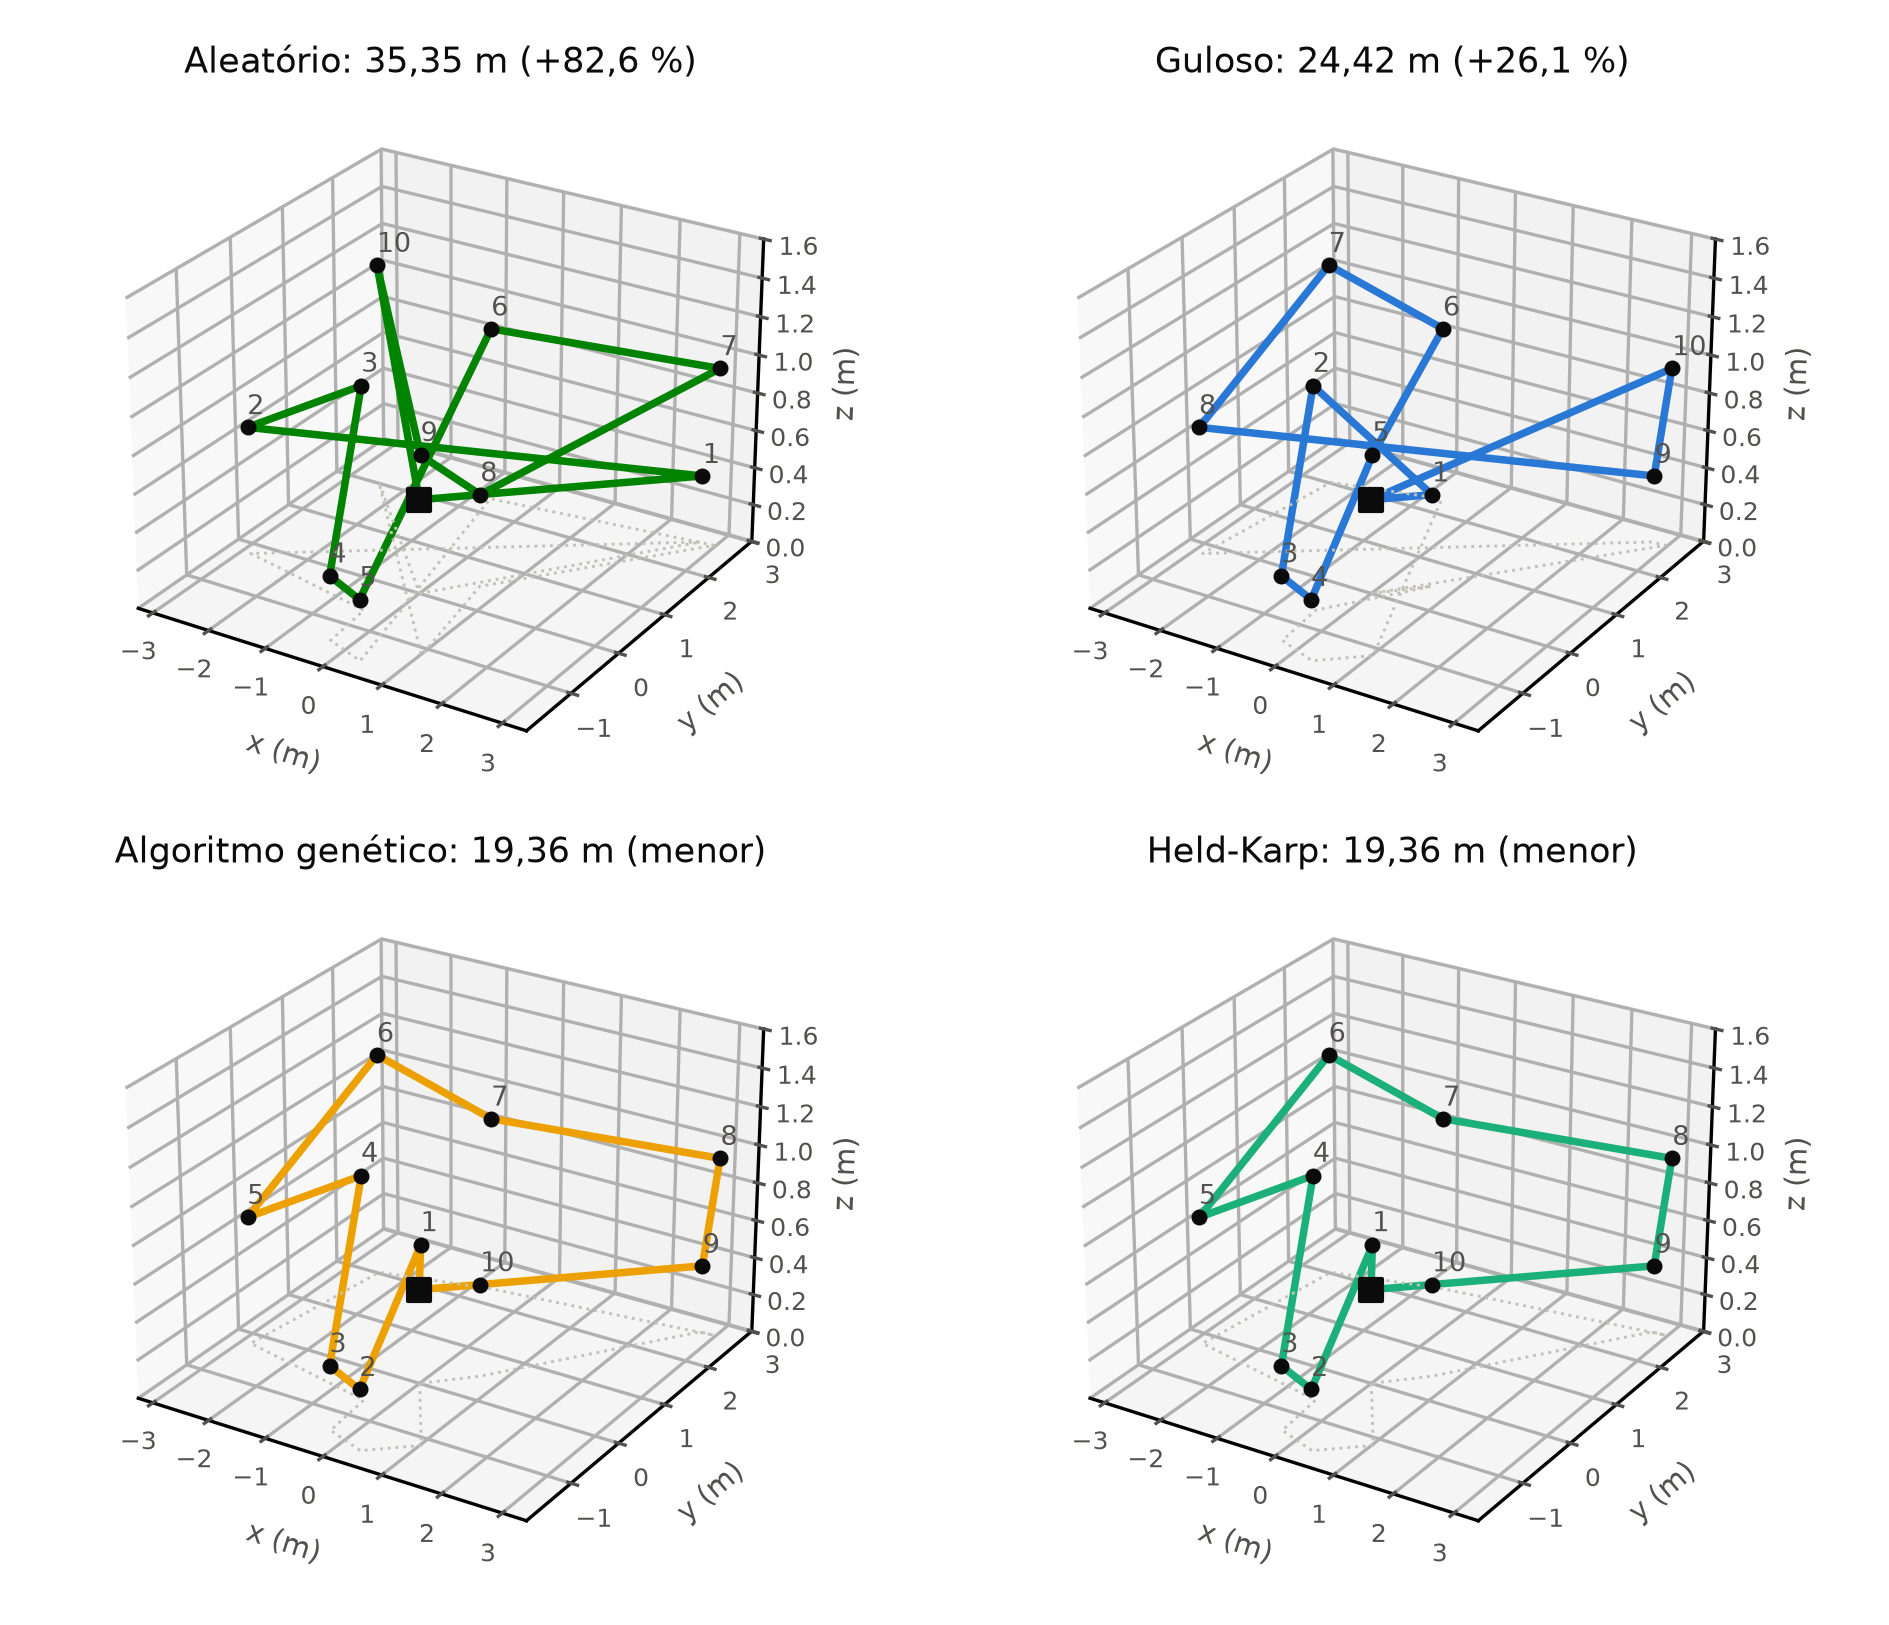
\includegraphics[width=\textwidth]{images/rotas/rotas_3d_n10.png}
    \fonte{elaborado pelos autores (2026).}
\end{figure}

\begin{figure}[H]
    \centering
    \caption{Rotas de 20 pontos obtidas pelos quatro algoritmos.}
    \label{fig:rotas_3d_n20}
    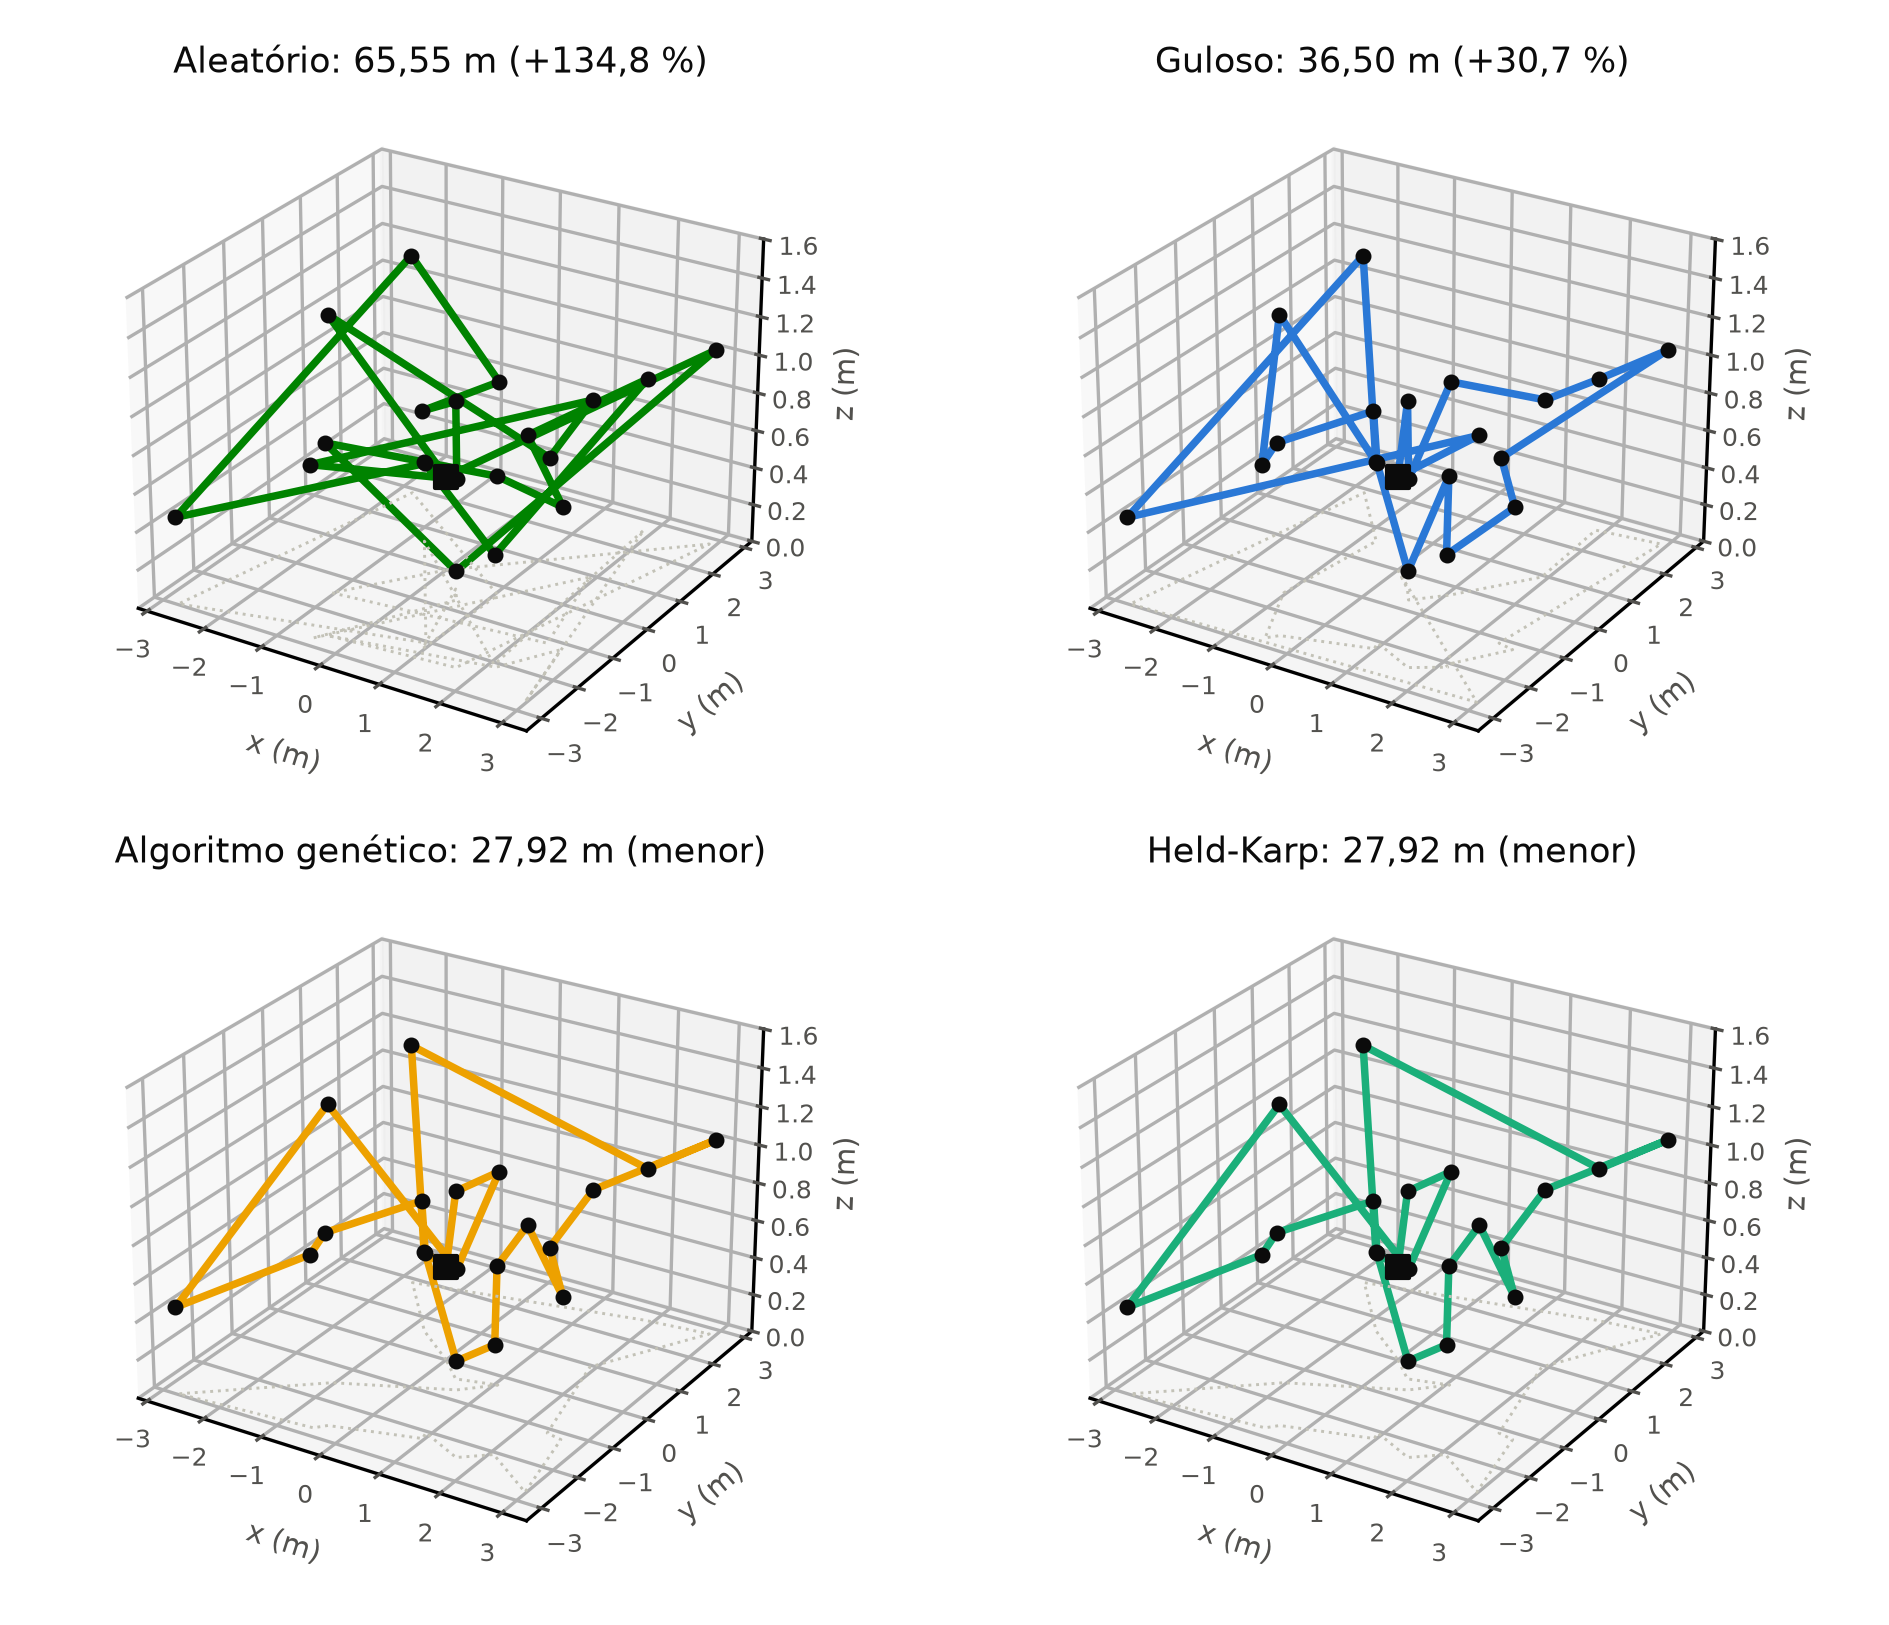
\includegraphics[width=\textwidth]{images/rotas/rotas_3d_n20.png}
    \fonte{elaborado pelos autores (2026).}
\end{figure}

\begin{figure}[H]
    \centering
    \caption{Rotas de 25 pontos, em que o Held-Karp não cabe na memória do computador.}
    \label{fig:rotas_3d_n25}
    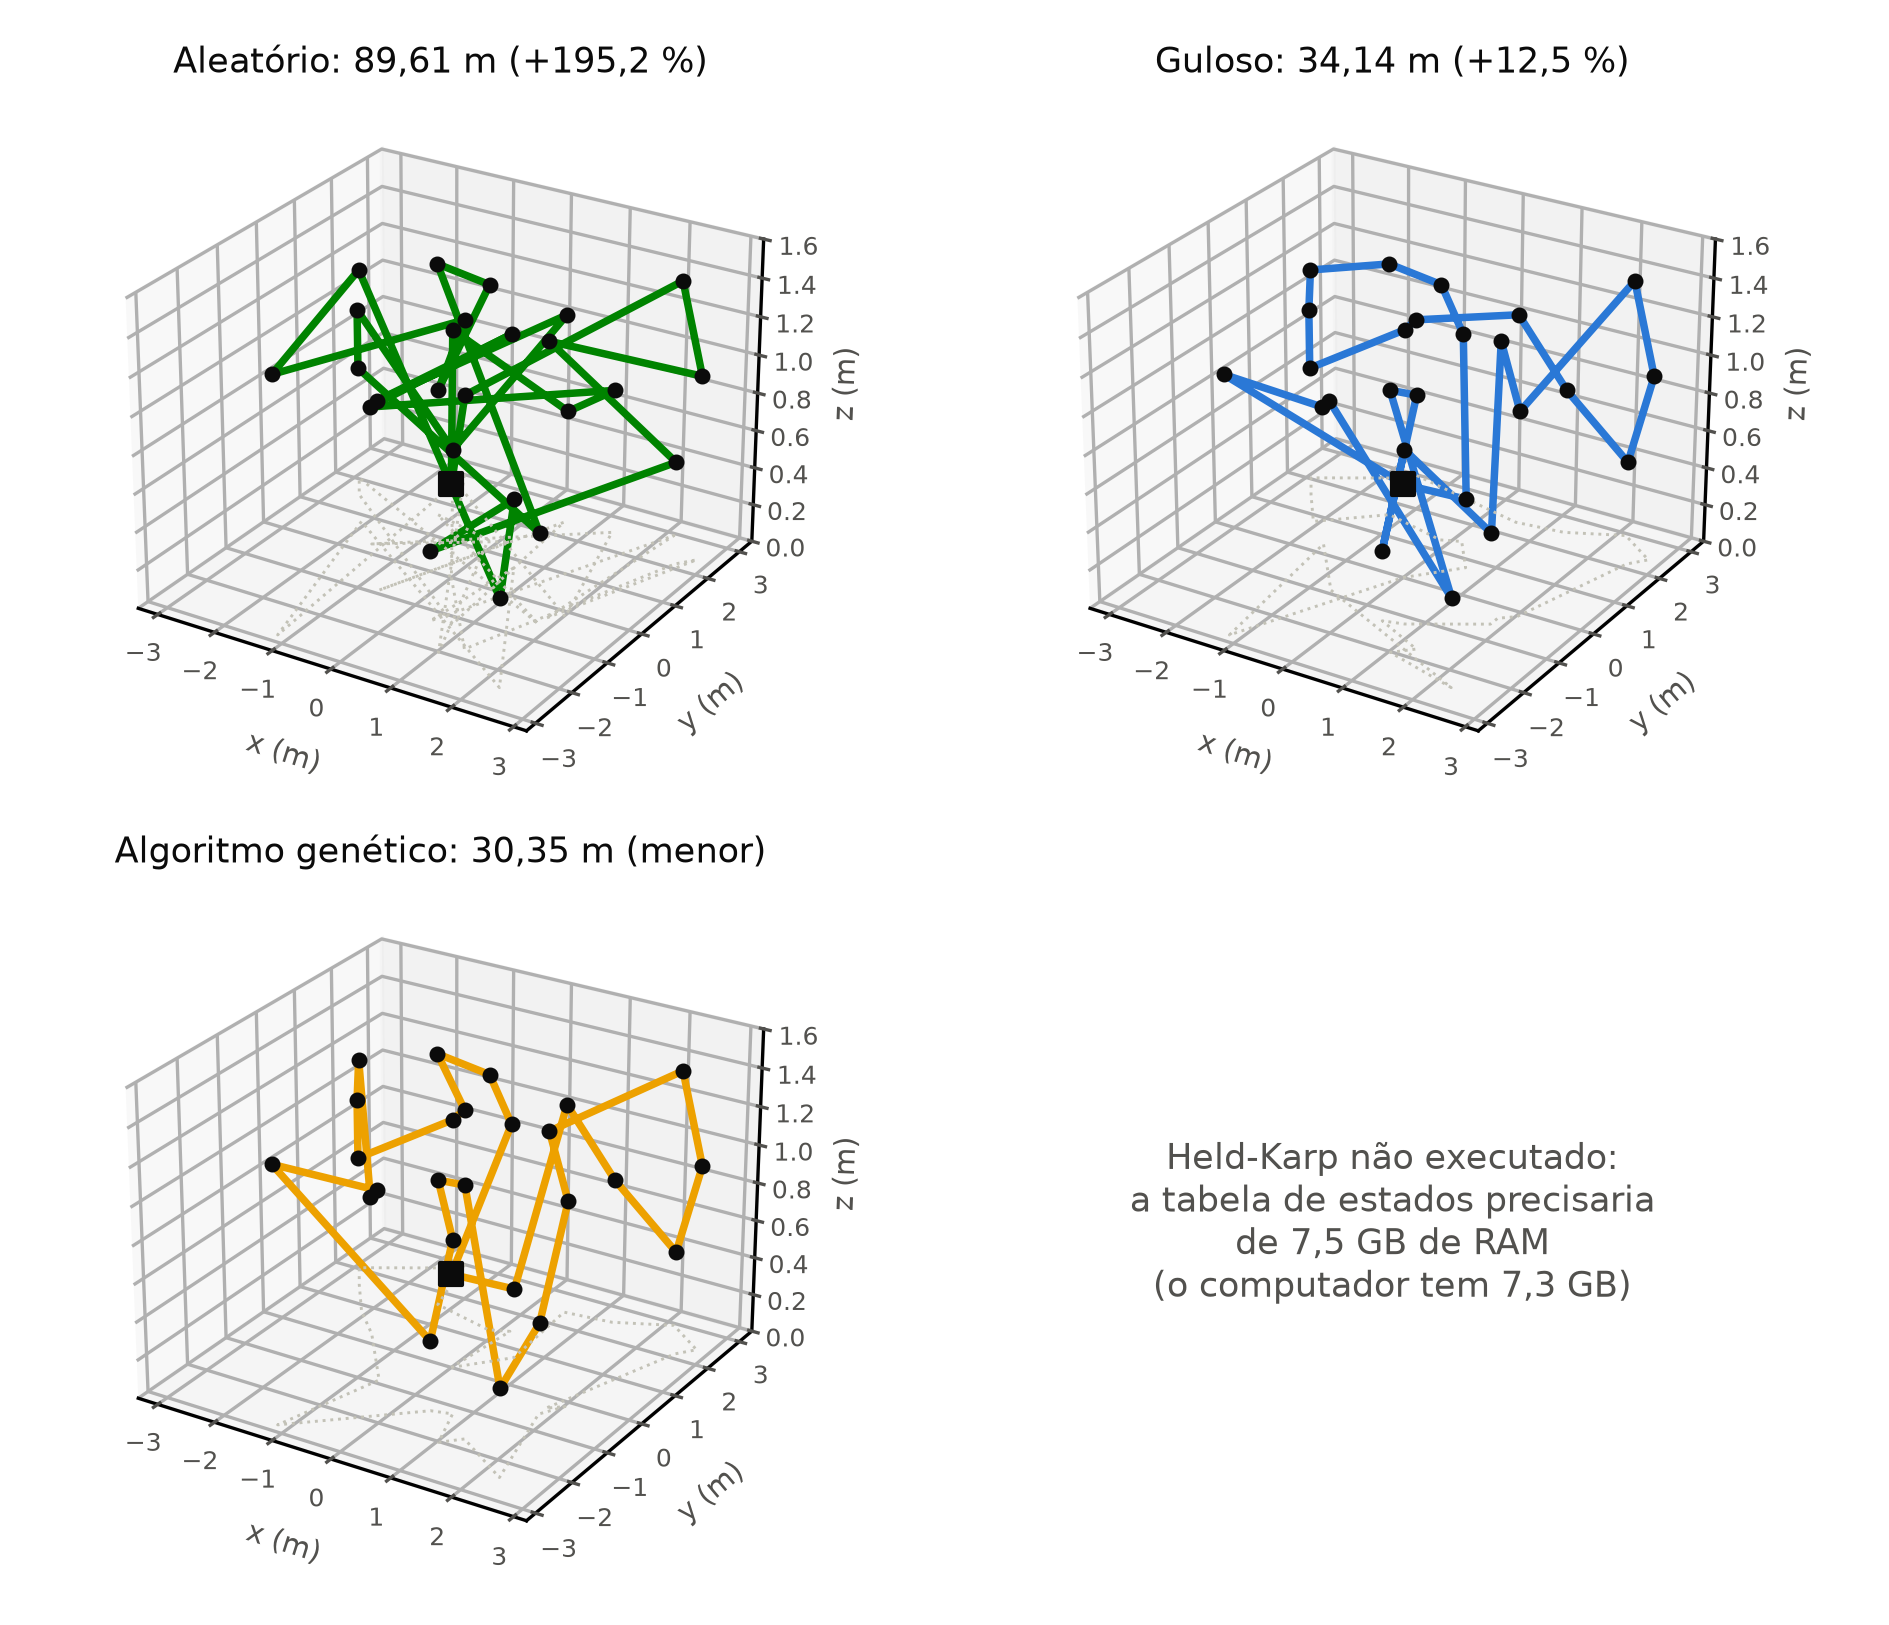
\includegraphics[width=\textwidth]{images/rotas/rotas_3d_n25.png}
    \fonte{elaborado pelos autores (2026).}
\end{figure}

% ----------------------------------------------------------------
\subsection{Tempo de cálculo}\label{subsec:res_rotas_tempo}
% ----------------------------------------------------------------

A Tabela~\ref{tab:rotas_tempo} apresenta o tempo médio de cálculo por instância no \textit{benchmark}. O AG levou de 0,13 a 0,45~s em toda a faixa, valor dominado pelo número de gerações (média de 272, mínimo de 200 e máximo de 665) e pouco sensível a $N$. A força bruta já é mais lenta que o AG com 10 pontos, e o Held-Karp, a partir de 15. Os tempos variaram cerca de 10\% entre execuções repetidas, conforme a carga do computador; as rotas e distâncias não se alteraram.

\begin{table}[H]
    \centering
    \caption{Tempo médio de cálculo por instância.}
    \label{tab:rotas_tempo}
    \small
    \renewcommand{\arraystretch}{1.2}
    \begin{tabular}{ccccc}
        \hline
        \textbf{$N$} & \textbf{Guloso} & \textbf{AG} & \textbf{Força bruta} & \textbf{Held-Karp} \\
        \hline
        5 & 0,03~ms & 139~ms & 0,06~ms & 0,07~ms \\
        10 & 0,07~ms & 162~ms & 1,56~s & 4,1~ms \\
        15 & 0,16~ms & 223~ms & --- & 260~ms \\
        20 & 0,25~ms & 281~ms & --- & 13,0~s \\
        22 & 0,32~ms & 282~ms & --- & 63,7~s \\
        25 & 0,39~ms & 376~ms & --- & --- \\
        30 & 0,54~ms & 454~ms & --- & --- \\
        \hline
    \end{tabular}
    \par\vspace{0.2cm}
    \footnotesize Fonte: elaborado pelos autores (2026).
\end{table}

% ----------------------------------------------------------------
\subsection{Convergência do algoritmo genético}\label{subsec:res_rotas_convergencia}
% ----------------------------------------------------------------

A Figura~\ref{fig:rotas_convergencia} mostra a evolução do melhor indivíduo do AG na primeira instância de quatro valores de $N$. A população inicial, aleatória, começa entre 35\% e 150\% acima da referência e melhora rapidamente nas primeiras 50 a 150 gerações, superando o guloso. Depois, a melhora cessa: com 10 e 20 pontos o AG atingiu o ótimo global, mas com 15 pontos estabilizou 3,4\% acima dele (24,27~m contra 23,47~m), preso em um ótimo local, isto é, uma rota que as operações do AG não conseguiram mais encurtar, embora existisse uma rota menor.

\begin{figure}[H]
    \centering
    \caption{Convergência do melhor indivíduo do algoritmo genético.}
    \label{fig:rotas_convergencia}
    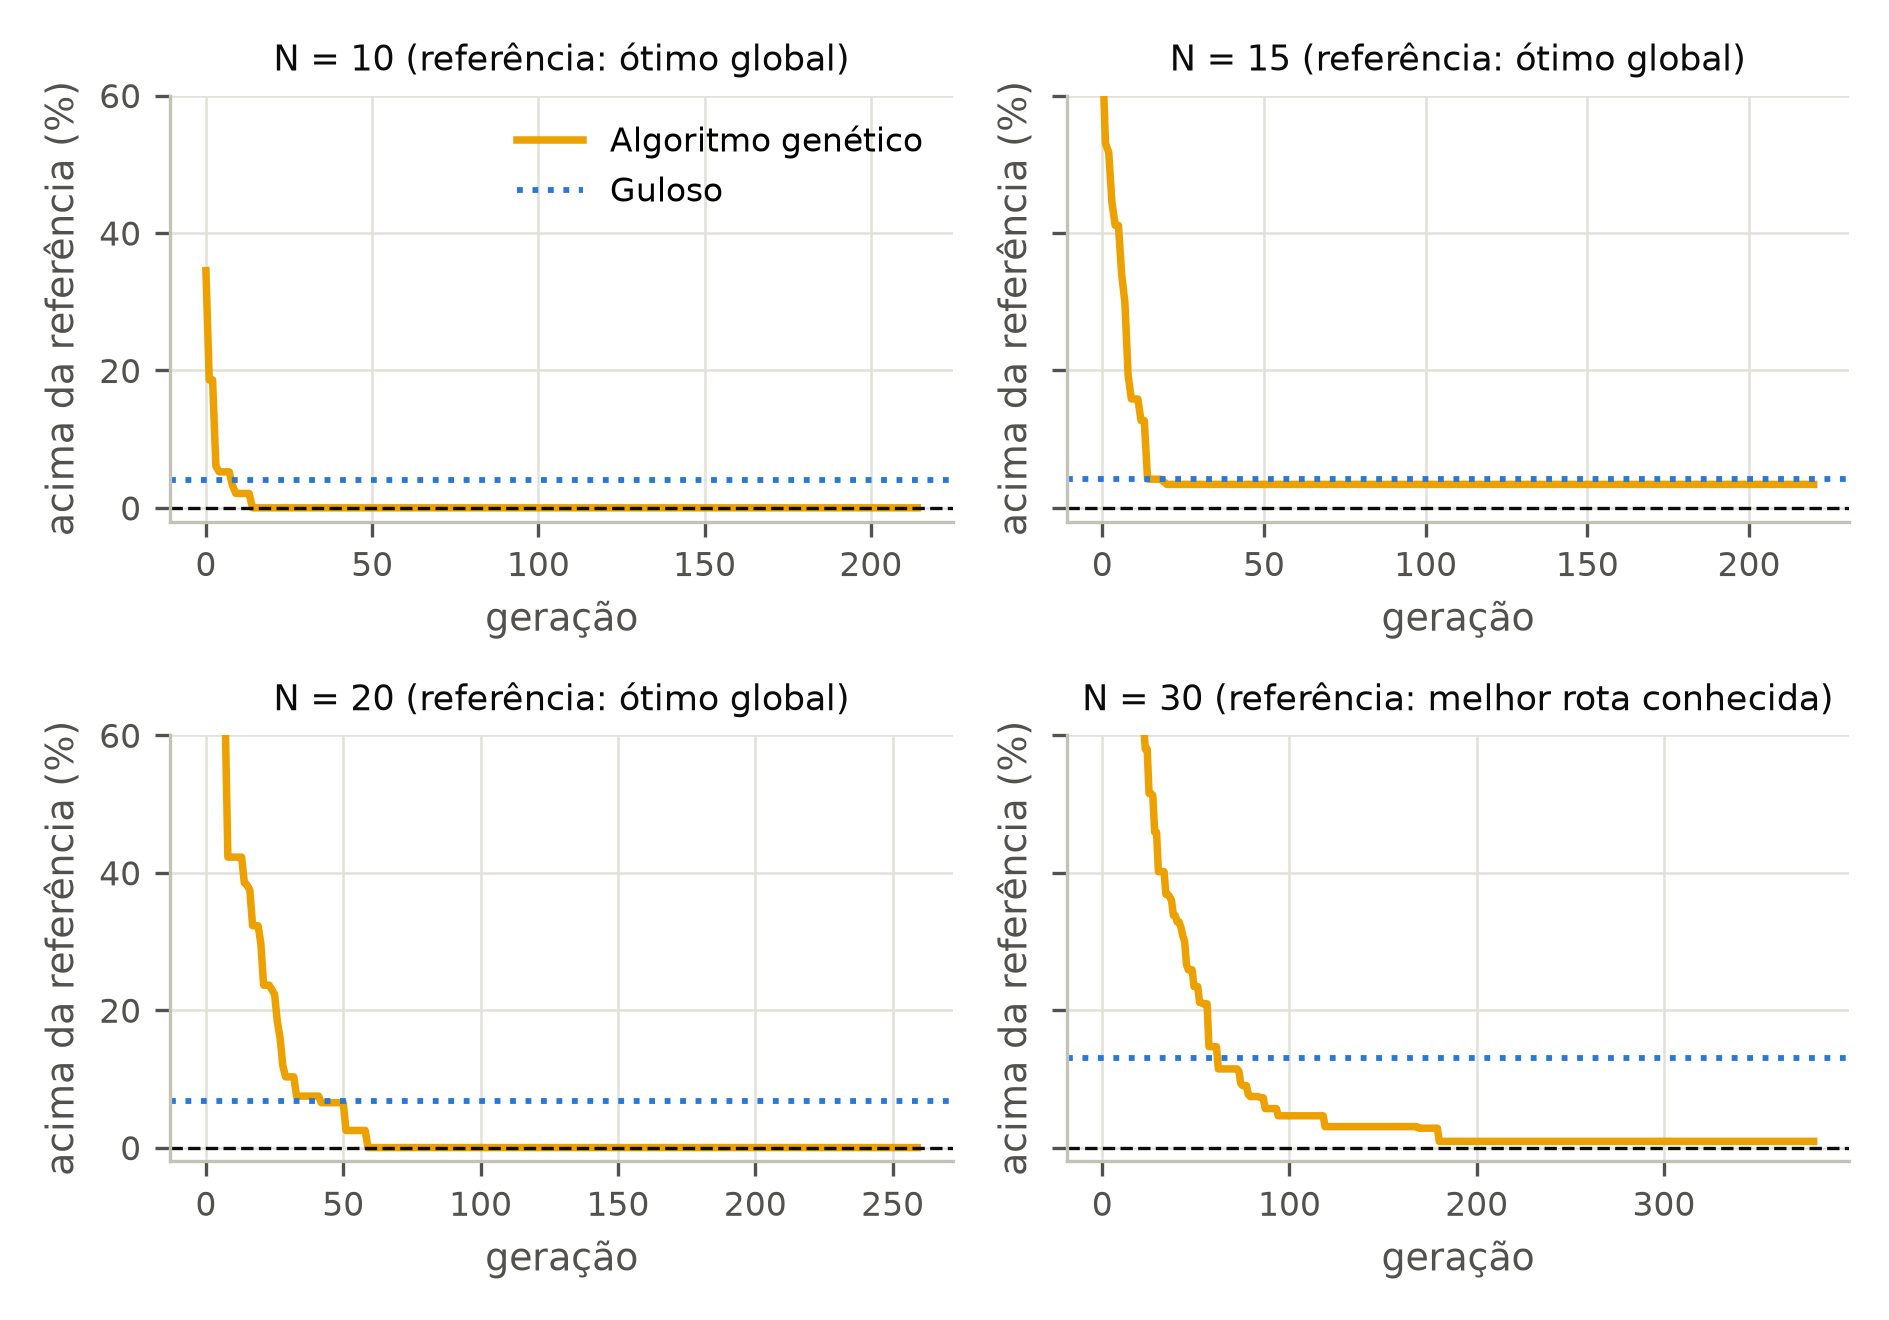
\includegraphics[width=\textwidth]{images/rotas/convergencia_genetico.png}
    \fonte{elaborado pelos autores (2026).}
\end{figure}

% ----------------------------------------------------------------
\subsection{Investigação complementar: busca local 2-opt}\label{subsec:res_rotas_2opt}
% ----------------------------------------------------------------

Durante o desenvolvimento, identificou-se na literatura que a busca local repetida a partir de várias rotas iniciais é uma alternativa competitiva para o TSP \cite{johnson1997}. Por isso, a busca local 2-opt com 20 partidas aleatórias foi incluída no \textit{benchmark} de forma exploratória, sem estudo aprofundado de seus parâmetros. A Tabela~\ref{tab:rotas_2opt} compara seus resultados com os do AG.

\begin{table}[H]
    \centering
    \caption{Comparação exploratória entre o AG e a busca local 2-opt com 20 partidas.}
    \label{tab:rotas_2opt}
    \small
    \renewcommand{\arraystretch}{1.25}
    \begin{tabular}{lcc}
        \hline
        \textbf{Indicador} & \textbf{AG} & \textbf{2-opt com 20 partidas} \\
        \hline
        Ótimo global obtido (instâncias de até 22 pontos) & 150 de 200 & 189 de 200 \\
        \textit{Gap} médio entre 11 e 22 pontos & 0,85\% & 0,04\% \\
        \textit{Gap} médio entre 23 e 30 pontos & 2,2\% & 0,05\% \\
        Tempo médio com 30 pontos & 454~ms & 16~ms \\
        Rota mais curta que a do outro (280 instâncias) & 8 & 106 \\
        \hline
    \end{tabular}
    \par\vspace{0.15cm}
    \footnotesize As 166 instâncias restantes terminaram empatadas.\\
    Fonte: elaborado pelos autores (2026).
\end{table}

Nos dados obtidos, a busca local com múltiplas partidas foi superior ao AG em qualidade e cerca de 30 vezes mais rápida. A análise das partidas ajuda a explicar o resultado: com 30 pontos, as 20 partidas convergiram em média para 18 ótimos locais diferentes, e somente 5,5\% delas alcançaram a melhor rota. Uma única busca local, portanto, fica facilmente presa em um ótimo local, mas repeti-la a partir de pontos de partida diferentes aumenta muito a chance de alcançar o ótimo global. Verificou-se também que 277 das 280 rotas do AG já eram ótimos locais em relação ao 2-opt; ou seja, o AG encontra ótimos locais com frequência, mas nem sempre o global. Como essa abordagem não foi estudada em profundidade, ela é indicada como alternativa a ser explorada em trabalhos futuros.

% ----------------------------------------------------------------
\subsection{Execução das rotas no controlador de voo}\label{subsec:res_rotas_stm32}
% ----------------------------------------------------------------

As rotas de uma instância tridimensional de 6 pontos, com alturas de 64 a 145~cm, foram executadas pelo STM32 com o VANT simulado, conforme a Seção~\ref{subsubsec:rotas_execucao_stm32} (Tabela~\ref{tab:rotas_stm32}). O AG obteve a mesma rota do Held-Karp percorrida no sentido inverso, com o mesmo comprimento, 21,3\% menor que a do guloso. Em todas as execuções, o VANT simulado chegou a cada ponto com erro máximo de 3,1~cm, dentro da tolerância de 5~cm usada pelo STM32 para declarar estabilidade.

\begin{table}[H]
    \centering
    \caption{Rotas tridimensionais executadas pelo STM32 com o VANT simulado.}
    \label{tab:rotas_stm32}
    \small
    \renewcommand{\arraystretch}{1.2}
    \begin{tabular}{ccccc}
        \hline
        \textbf{Algoritmo} & \textbf{Ordem} & \textbf{Circuito 3D} & \textbf{Trechos executados} & \textbf{Maior erro em um ponto} \\
        \hline
        Guloso & 3 4 5 2 1 6 & 1898~cm & 14 & 3,0~cm \\
        AG & 3 4 6 5 2 1 & 1493~cm ($-21{,}3\%$) & 14 & 3,0~cm \\
        Held-Karp & 1 2 5 6 4 3 & 1493~cm ($-21{,}3\%$) & 14 & 3,1~cm \\
        \hline
    \end{tabular}
    \par\vspace{0.15cm}
    \footnotesize Pontos (cm): $(-177, 188, 129)$, $(-104, -150, 145)$, $(43, -43, 99)$, $(62, -71, 64)$, $(92, -204, 93)$ e $(298, -274, 134)$.\\
    Fonte: elaborado pelos autores (2026).
\end{table}

% ----------------------------------------------------------------
\subsection{Execução do algoritmo genético no Raspberry Pi Zero W}\label{subsec:res_rotas_pi}
% ----------------------------------------------------------------

A Tabela~\ref{tab:rotas_pi} compara a rota obtida pelo AG no computador pessoal e no Raspberry Pi Zero W para três instâncias: o quadrado de 40~cm executado com o VANT simulado no STM32 no ensaio de comunicação (Seção~\ref{subsec:res_com_missao}) e duas instâncias do \textit{benchmark}, com 10 e 30 pontos. Nas três, a ordem, o comprimento e a assinatura SHA-256 foram idênticos nas duas máquinas: o Raspberry Pi calcula exatamente a mesma rota, e os resultados de qualidade do \textit{benchmark} valem para o algoritmo embarcado. Os 26 testes automatizados do programa também foram aprovados no próprio Raspberry Pi.

\begin{table}[H]
    \centering
    \caption{Mesma rota calculada pelo AG no computador pessoal e no Raspberry Pi Zero W.}
    \label{tab:rotas_pi}
    \small
    \renewcommand{\arraystretch}{1.2}
    \begin{tabular}{lccccc}
        \hline
        \textbf{Instância} & \textbf{Comprimento} & \textbf{SHA-256} & \textbf{PC} & \textbf{Raspberry Pi} & \textbf{Razão} \\
        \hline
        Quadrado de 40~cm & 160,0~cm & \texttt{52d2b0c4\ldots} & 0,14~s & 9,70~s & 69$\times$ \\
        10 pontos & 19,36~m & \texttt{9ffc5830\ldots} & 0,16~s & 11,14~s & 70$\times$ \\
        30 pontos & 30,84~m & \texttt{11f260a1\ldots} & 0,39~s & 23,92~s & 61$\times$ \\
        \hline
    \end{tabular}
    \par\vspace{0.15cm}
    \footnotesize A assinatura é a mesma nas duas máquinas; são mostrados os 8 primeiros dígitos hexadecimais. Tempos de uma execução de cada instância.\\
    Fonte: elaborado pelos autores (2026).
\end{table}

O Raspberry Pi foi de 61 a 70 vezes mais lento, levando de 10 a 24~s para ordenar de 3 a 30 pontos. Como a ordem é calculada uma única vez, antes da execução da rota, e cada trecho leva vários segundos para ser voado, esse tempo é aceitável para a aplicação. Os métodos exatos, por outro lado, seriam ainda mais limitados na placa: além de dezenas de vezes mais lentos, o Held-Karp ultrapassa metade dos 512~MB de RAM a partir de 21 pontos (Seção~\ref{subsec:res_rotas_limite}).

% ----------------------------------------------------------------
\subsection{Discussão}\label{subsec:res_rotas_discussao}
% ----------------------------------------------------------------

Os resultados confirmam que a obtenção do ótimo global se torna inviável com poucas dezenas de pontos, mesmo com o melhor dos métodos exatos avaliados. A força bruta, que traduz diretamente a definição do problema, deixa de ser praticável com 11 pontos. O Held-Karp estende esse limite para 22 pontos, sendo cerca de $10^{11}$ vezes mais rápido que a força bruta com 20 pontos, ao custo de uma tabela de estados que dobra a cada ponto adicionado; com 25 pontos, a memória necessária excede a do computador utilizado e, no Raspberry Pi Zero W, o limite é ainda menor.

O algoritmo genético manteve tempo inferior a 0,5~s e memória inferior a 0,1~MB em toda a faixa, com rotas iguais ao ótimo até 10 pontos e, em média, até 3,7\% acima da referência nas faixas maiores. Isso o torna viável exatamente onde os métodos exatos deixam de ser, e o \textit{benchmark} nas faixas em que o ótimo é conhecido fundamenta o uso de sua rota quando o ótimo não pode ser calculado. O guloso, embora mais rápido, perdeu de 6\% a 18\% de distância em média, e a ordem aleatória chegou a três vezes o comprimento ótimo.

No Raspberry Pi Zero W, o mesmo AG produziu exatamente as mesmas rotas, com tempo de 10 a 24~s, de 60 a 70 vezes maior que no computador pessoal. Esses resultados sustentam a viabilidade do algoritmo genético como solução adotada e validada no projeto, com qualidade de rota e tempo de cálculo compatíveis com o planejamento antes do voo. A validação de sua execução no Raspberry Pi e da integração com o controlador de voo fundamenta sua utilização no protótipo, mas não demonstra superioridade em relação a todas as alternativas avaliadas.

Um limite deve ser considerado: o AG implementado não usa busca local, ou seja, não tenta encurtar as rotas por pequenas modificações sistemáticas, e pode estabilizar em um ótimo local, como observado com 15 pontos. A investigação complementar indicou que a busca local repetida obteve rotas melhores em menos tempo; combiná-la ao AG, formando um algoritmo memético \cite{moscato1989}, ou adotá-la diretamente são caminhos para trabalhos futuros.
